% Options for packages loaded elsewhere
\PassOptionsToPackage{unicode}{hyperref}
\PassOptionsToPackage{hyphens}{url}
%
\documentclass[
  12pt,
]{article}
\usepackage{lmodern}
\usepackage{amssymb,amsmath}
\usepackage{ifxetex,ifluatex}
\ifnum 0\ifxetex 1\fi\ifluatex 1\fi=0 % if pdftex
  \usepackage[T1]{fontenc}
  \usepackage[utf8]{inputenc}
  \usepackage{textcomp} % provide euro and other symbols
\else % if luatex or xetex
  \usepackage{unicode-math}
  \defaultfontfeatures{Scale=MatchLowercase}
  \defaultfontfeatures[\rmfamily]{Ligatures=TeX,Scale=1}
\fi
% Use upquote if available, for straight quotes in verbatim environments
\IfFileExists{upquote.sty}{\usepackage{upquote}}{}
\IfFileExists{microtype.sty}{% use microtype if available
  \usepackage[]{microtype}
  \UseMicrotypeSet[protrusion]{basicmath} % disable protrusion for tt fonts
}{}
\makeatletter
\@ifundefined{KOMAClassName}{% if non-KOMA class
  \IfFileExists{parskip.sty}{%
    \usepackage{parskip}
  }{% else
    \setlength{\parindent}{0pt}
    \setlength{\parskip}{6pt plus 2pt minus 1pt}}
}{% if KOMA class
  \KOMAoptions{parskip=half}}
\makeatother
\usepackage{xcolor}
\IfFileExists{xurl.sty}{\usepackage{xurl}}{} % add URL line breaks if available
\IfFileExists{bookmark.sty}{\usepackage{bookmark}}{\usepackage{hyperref}}
\hypersetup{
  hidelinks,
  pdfcreator={LaTeX via pandoc}}
\urlstyle{same} % disable monospaced font for URLs
\usepackage[margin=1in]{geometry}
\usepackage{graphicx,grffile}
\makeatletter
\def\maxwidth{\ifdim\Gin@nat@width>\linewidth\linewidth\else\Gin@nat@width\fi}
\def\maxheight{\ifdim\Gin@nat@height>\textheight\textheight\else\Gin@nat@height\fi}
\makeatother
% Scale images if necessary, so that they will not overflow the page
% margins by default, and it is still possible to overwrite the defaults
% using explicit options in \includegraphics[width, height, ...]{}
\setkeys{Gin}{width=\maxwidth,height=\maxheight,keepaspectratio}
% Set default figure placement to htbp
\makeatletter
\def\fps@figure{htbp}
\makeatother
\setlength{\emergencystretch}{3em} % prevent overfull lines
\providecommand{\tightlist}{%
  \setlength{\itemsep}{0pt}\setlength{\parskip}{0pt}}
\setcounter{secnumdepth}{-\maxdimen} % remove section numbering
\usepackage{setspace}\doublespacing
\usepackage{float}
\usepackage{caption}
\usepackage{booktabs}
\usepackage{longtable}
\usepackage{array}
\usepackage{multirow}
\usepackage{wrapfig}
\usepackage{float}
\usepackage{colortbl}
\usepackage{pdflscape}
\usepackage{tabu}
\usepackage{threeparttable}
\usepackage{threeparttablex}
\usepackage[normalem]{ulem}
\usepackage{makecell}
\usepackage{xcolor}

\author{}
\date{\vspace{-2.5em}}

\begin{document}

\captionsetup[figure]{labelformat=empty}
\captionsetup[table]{labelformat=empty}
\renewcommand{\figurename}{}

\hypertarget{supporting-information}{%
\section{Supporting information:}\label{supporting-information}}

\hypertarget{recipient-and-donor-characteristics-govern-the-hierarchical-structure-of-heterospecific-pollen-competition-networks}{%
\section{Recipient and donor characteristics govern the hierarchical
structure of heterospecific pollen competition
networks}\label{recipient-and-donor-characteristics-govern-the-hierarchical-structure-of-heterospecific-pollen-competition-networks}}

\textbf{Authors:} Jose B. Lanuza, Ignasi Bartomeus, Tia Lynn Ashman,
Romina Rader

The following Supporting Information is available for this article:

\textbf{Table S1.} Species names, common names, varieties and sources of
the different seeds.

\textbf{Table S2.} Numerical values of all the traits measured for each
species.

\textbf{Table S3.} Seed set in percentage for hand cross-pollination,
hand self-pollination, natural selfing and apomixis for all species.

\textbf{Table S4.} Species x species matrix with the significance of
effect ``yes'' or ``no'' of the different donors on the seed set of the
different recipient species.

\textbf{Table S5.} Estimates, standard error, t-value and P-value of the
effect of the different 9 donors on each recipient species.

\textbf{Table S6.} Number of seeds produced with 100\% foreign pollen
treatments for the different recipient species.

\textbf{Table S7.} Phylogenetic signal and significance for all the
different traits

\textbf{Table S8.} Procrustes analysis results.

\textbf{Figure S1}. Total amount of pollen deposited per stigma.

\textbf{Figure S2}. Pollen ratios for the different recipient species.

\textbf{Figure S3}. Pollen ratios for the different recipient species by
family.

\textbf{Figure S4}. Statistical comparison of the pollen ratios by
family.

\textbf{Figure S5}. Unipartite bidirectional network with asymmetrical
effect.

\textbf{Figure S6}. Correlation matrix for all the different traits.

\textbf{Figure S7}. Species reproductive biology.

\textbf{Figure S8}. Grouped effect sizes by family for each recipient
species.

\newpage

\#TABLE S1 \begingroup\fontsize{7}{9}\selectfont

\begin{longtabu} to \linewidth {>{\raggedright}X>{\raggedright}X>{\raggedright}X>{\raggedright}X}
\toprule
\textbf{Species} & \textbf{Common\_names} & \textbf{Variety} & \textbf{Source}\\
\midrule
\endfirsthead
\multicolumn{4}{@{}l}{\textit{(continued)}}\\
\toprule
Species & Common\_names & Variety & Source\\
\midrule
\endhead
\
\endfoot
\bottomrule
\endlastfoot
\rowcolor{gray!6}  Brassica oleracea & Wild cabbage & Capitata & https://www.mrfothergills.com.au/\\
\addlinespace
Brassica rapa & Pak choi & Chinensis & https://www.mrfothergills.com.au/\\
\addlinespace
\rowcolor{gray!6}  Eruca sativa & Rocket &  & https://www.mrfothergills.com.au/\\
\addlinespace
Sinapis alba & White mustard &  & https://www.mrfothergills.com.au/\\
\addlinespace
\rowcolor{gray!6}  Ipomoea aquatica & Water spinach &  & https://www.theseedcollection.com.au/\\
\addlinespace
Ipomoea purpurea & Morning glory &  & http://www.shaman-australis.com.au\\
\addlinespace
\rowcolor{gray!6}  Capsicum annuum & Capsicum & California Wonder & https://www.edenseeds.com.au\\
\addlinespace
Petunia integrifolia & Petunia &  & https://www.dianeseeds.com/\\
\addlinespace
\rowcolor{gray!6}  Solanum lycopersicum & Tomato & Tommy Toe & https://www.mrfothergills.com.au/\\
\addlinespace
Solanum melongena & Eggplant & Little Fingers & https://www.4seasonsseeds.com.au/\\*
\end{longtabu}
\endgroup{}

\begin{landscape}

TABLE S2
\begingroup\fontsize{6}{8}\selectfont

\resizebox{\linewidth}{!}{
\begin{tabu} to \linewidth {>{\raggedright\arraybackslash}p{2cm}>{\raggedleft}X>{\raggedleft}X>{\raggedleft}X>{\raggedleft}X>{\raggedleft}X>{\raggedleft}X>{\raggedleft}X>{\raggedleft}X>{\raggedleft}X>{\raggedleft}X>{\raggedleft}X>{\raggedleft}X>{\raggedleft}X}
\toprule
\textbf{Species} & \textbf{Pollen size $\mu$m} & \textbf{Pollen grains per anther} & \textbf{Ovule number} & \textbf{Pollen:ovule ratio} & \textbf{Stigma area $\mu$m$^{2}$} & \textbf{Stigma length (mm)} & \textbf{Stigma width (mm)} & \textbf{Style length (mm)} & \textbf{Style width (mm)} & \textbf{Ovary length (mm)} & \textbf{Ovary width (mm)} & \textbf{Selfing rate} & \textbf{SI index}\\
\midrule
\rowcolor{gray!6}  Brassica oleracea & 27.72 & 42033 & 29 & 8696.48 & 0.62 & 0.53 & 0.88 & 2.32 & 0.65 & 5.93 & 1.11 & 0.0 & 0.00\\
\addlinespace
Brassica rapa & 25.35 & 7133 & 26 & 1646.08 & 0.36 & 0.37 & 0.73 & 1.08 & 0.52 & 3.53 & 0.88 & 0.0 & 0.00\\
\addlinespace
\rowcolor{gray!6}  Capsicum annuum & 32.46 & 30761 & 241 & 765.83 & 1.06 & 0.72 & 1.18 & 3.24 & 1.06 & 3.15 & 5.80 & 0.8 & 0.64\\
\addlinespace
Eruca versicaria & 24.95 & 22151 & 24 & 5537.75 & 0.35 & 0.73 & 0.67 & 6.60 & 0.73 & 4.42 & 0.94 & 0.1 & 0.02\\
\addlinespace
\rowcolor{gray!6}  Ipomoea aquatica & 70.10 & 858 & 4 & 1072.50 & 3.26 & 1.43 & 2.25 & 19.44 & 0.45 & 2.38 & 1.42 & 0.6 & 0.75\\
\addlinespace
Ipomoea purpurea & 97.59 & 654 & 6 & 545.00 & 2.27 & 1.24 & 1.88 & 28.23 & 0.58 & 1.06 & 1.57 & 1.0 & 2.74\\
\addlinespace
\rowcolor{gray!6}  Petunia integrifolia & 24.74 & 34657 & 220 & 787.66 & 1.17 & 0.80 & 1.32 & 14.65 & 0.45 & 3.13 & 1.77 & 0.9 & 0.26\\
\addlinespace
Sinapis alba & 33.59 & 3507 & 6 & 3507.00 & 0.55 & 0.63 & 0.91 & 3.62 & 0.77 & 1.98 & 1.07 & 0.7 & 1.12\\
\addlinespace
\rowcolor{gray!6}  Solanum lycopersicum & 22.00 & 28915 & 92 & 1885.76 & 0.09 & 0.19 & 0.35 & 6.47 & 0.31 & 1.16 & 1.13 & 0.7 & 0.48\\
\addlinespace
Solanum melongena & 25.18 & 166989 & 1010 & 992.01 & 1.14 & 0.96 & 1.33 & 11.33 & 0.94 & 4.02 & 3.55 & 1.0 & 1.45\\
\bottomrule
\end{tabu}}
\endgroup{}

\end{landscape}

TABLE S3 \begingroup\fontsize{6}{8}\selectfont

\resizebox{\linewidth}{!}{
\begin{tabu} to \linewidth {>{\raggedright\arraybackslash}p{2cm}>{\raggedleft}X>{\raggedleft}X>{\raggedleft}X>{\raggedleft}X}
\toprule
\textbf{Species} & \textbf{Hand cross-pollination} & \textbf{Hand self-pollination} & \textbf{Spontaneous selfing} & \textbf{Apomixis}\\
\midrule
\rowcolor{gray!6}  Brassica oleracea & 32.07 & 0.00 & 0.00 & 0\\
\addlinespace
Brassica rapa & 44.97 & 0.00 & 0.00 & 0\\
\addlinespace
\rowcolor{gray!6}  Capsicum annuum & 80.00 & 56.47 & 19.34 & 0\\
\addlinespace
Eruca sativa & 23.75 & 0.42 & 0.00 & 0\\
\addlinespace
\rowcolor{gray!6}  Ipomoea aquatica & 40.00 & 30.00 & 20.00 & 0\\
\addlinespace
Ipomoea purpurea & 31.67 & 86.67 & 31.67 & 0\\
\addlinespace
\rowcolor{gray!6}  Petunia integrifolia & 80.16 & 24.77 & 0.00 & 0\\
\addlinespace
Sinapis alba & 41.67 & 48.33 & 5.00 & 15\\
\addlinespace
\rowcolor{gray!6}  Solanum lycopersium & 85.65 & 41.20 & 68.48 & 0\\
\addlinespace
Solanum melongena & 60.48 & 74.87 & 21.56 & 0\\
\bottomrule
\end{tabu}}
\endgroup{}

\newpage

\begin{figure}
\centering
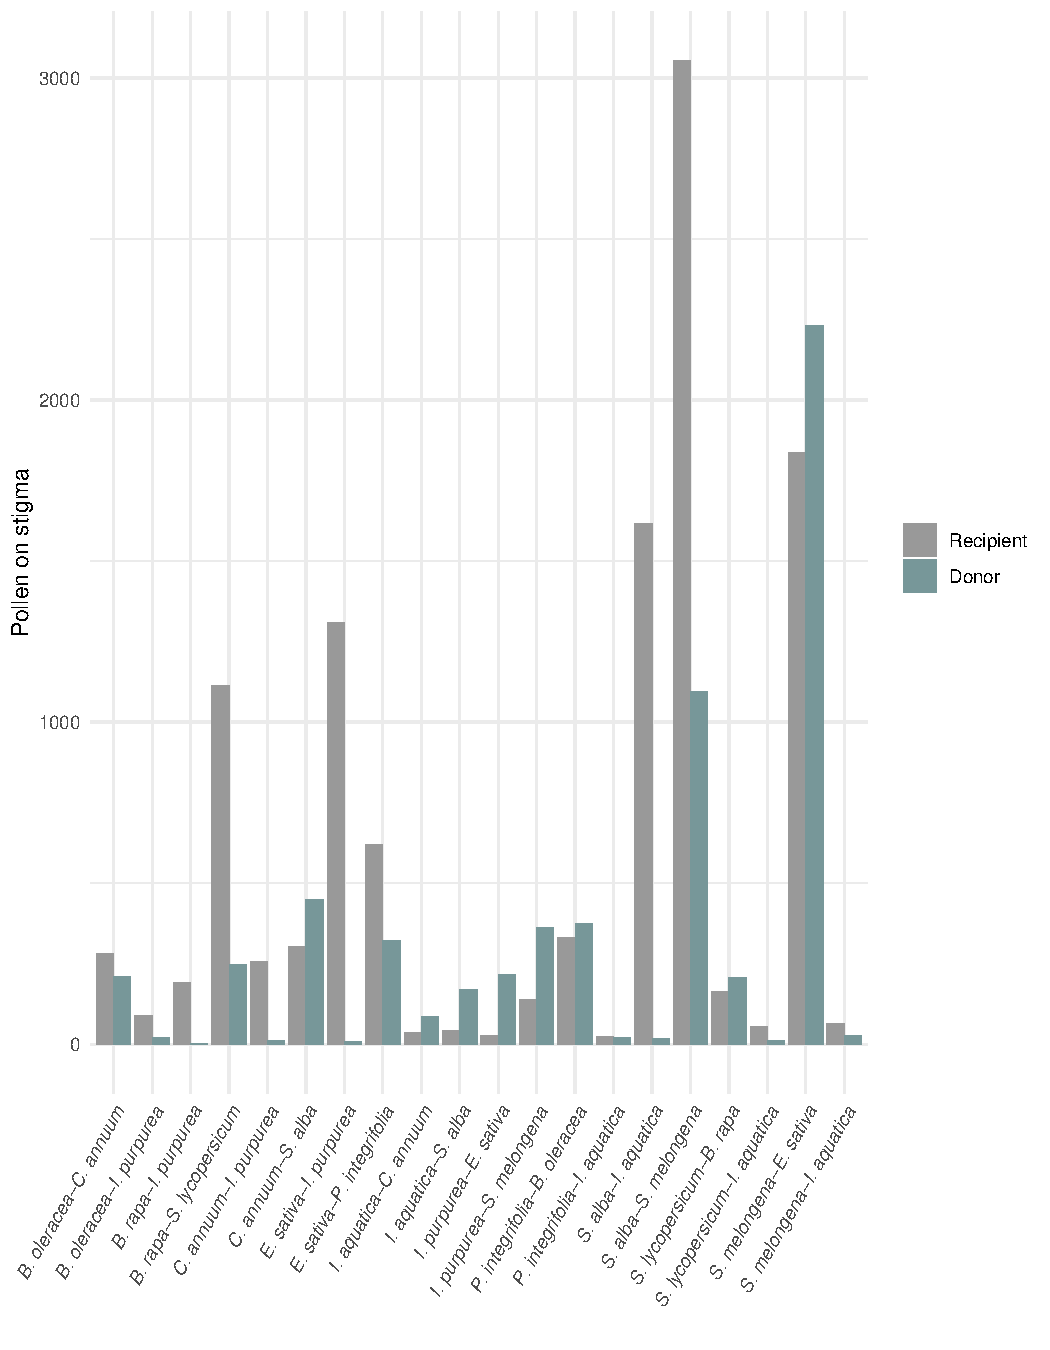
\includegraphics{Supp_Material_files/figure-latex/unnamed-chunk-4-1.pdf}
\caption{\textbf{Fig. S1} Average number of pollen grains per stigma for
20 different treatments (3 replicates per tratment). For each treatment,
we show the average number of conspecific pollen grains (grey) and
heterospecific pollen grains (light blue) per stigma. For each pair of
species on the x-axis, the first species is the recipient species, and
the second, the donor species.}
\end{figure}

\clearpage

\begin{figure}
\centering
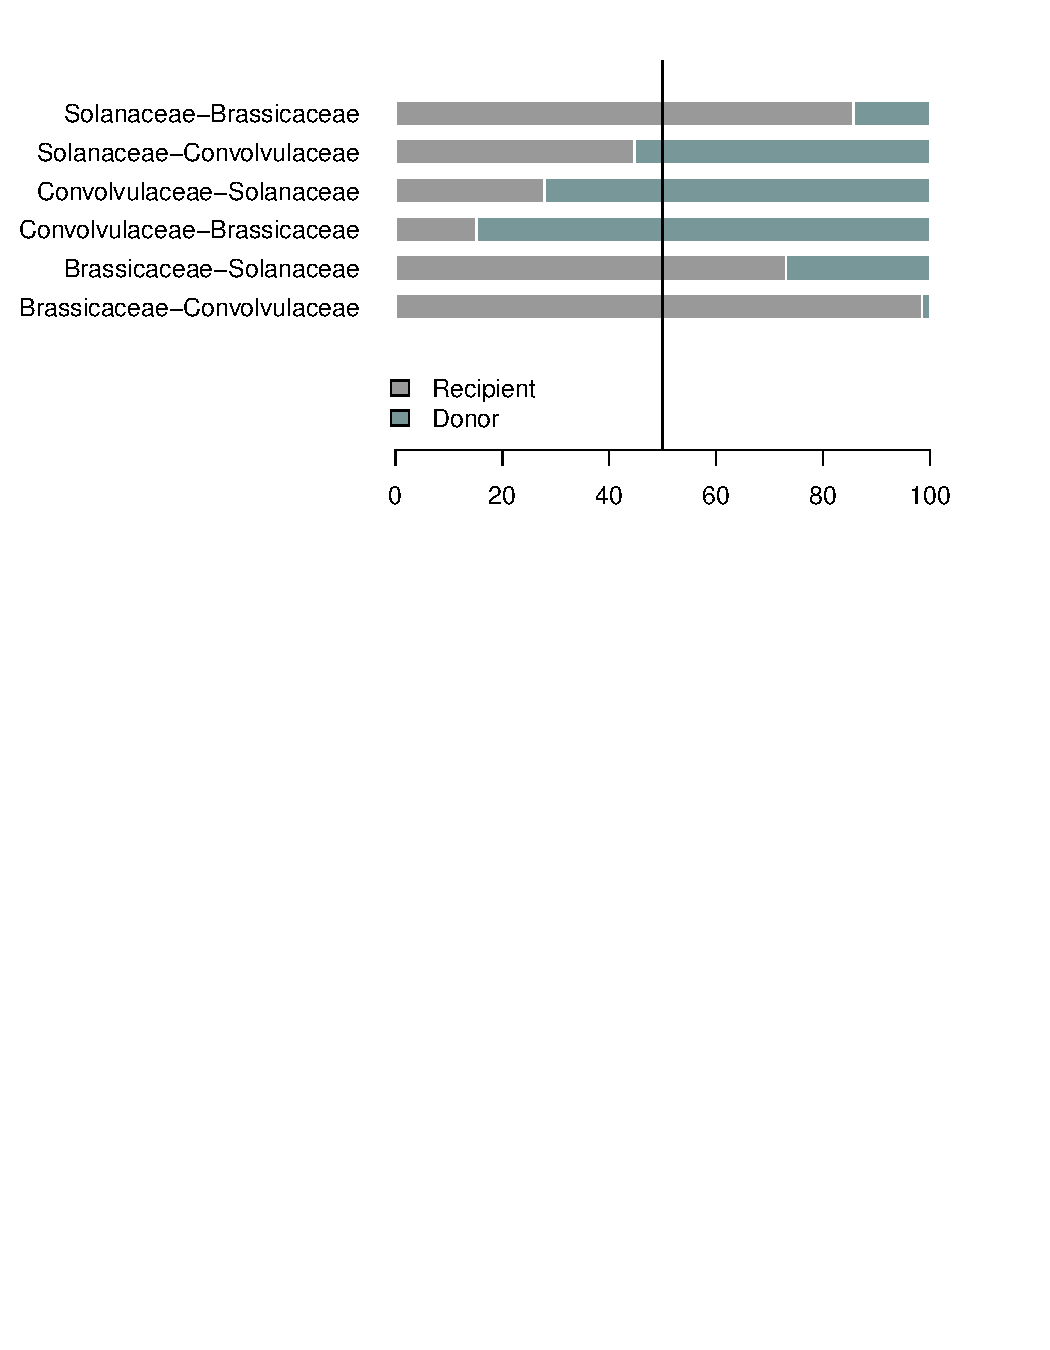
\includegraphics{Supp_Material_files/figure-latex/unnamed-chunk-5-1.pdf}
\caption{\textbf{Fig. S2} Average proportion of conspecific and
heterospecific pollen per stigma grouped by family, A) Brassicaceae, B)
Solanaceae and C) Convolvulaceae. These proportions (\%) are the number
of conspecific pollen grains or heterospecific pollen grains divided by
the total number of pollen grains per stigma for 20 different
treatments. We conducted 3 count replicates per treatment and then we
calculated the average number of pollen grains for these treatments. The
proportion of conspecific and heterospecific pollen are shown in grey
and light blue respectively. For each pair of species on the y-axis, the
first species is the pollen recipient and the second the pollen donor.
The vertical black line represents 50\% pollen of both donor and
recipient.}
\end{figure}

\clearpage

\begin{figure}
\centering
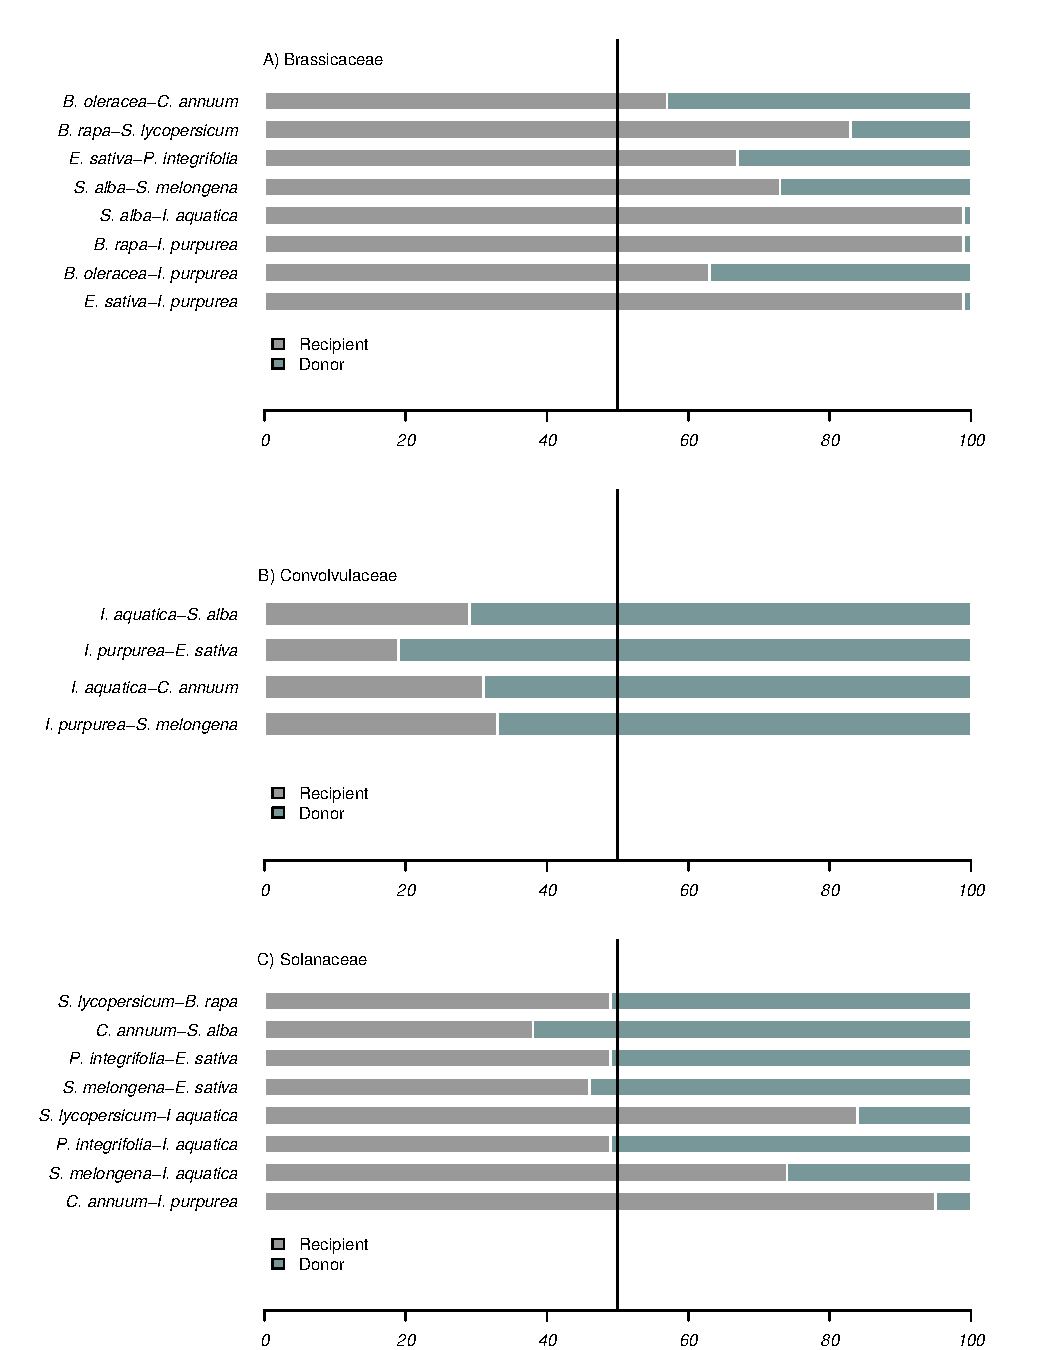
\includegraphics{Supp_Material_files/figure-latex/unnamed-chunk-6-1.pdf}
\caption{\textbf{Fig. S3} Average proportion (\%) of heterospecific and
conspecific pollen per family for the different 20 treatments counted.
We conducted 3 count replicates per treatment and then we calculated the
average number of pollen grains for these different 20 treatments.
Finally, we grouped by family these treatments in order to see general
tendencies across families as pollen donor and as pollen recipient.
Pollen ratios were considered as the number of conspecific or
heterospecific pollen grains divided by the total number of pollen
grains per stigma. On the y-axis, the first family on each pair of plant
families is the recipient one, and the second, the family of the donor.
The vertical bar on intercept 50, represents equal proportions of both
recipient (grey) and donor (light blue) pollen.}
\end{figure}

\clearpage

\begin{figure}
\centering
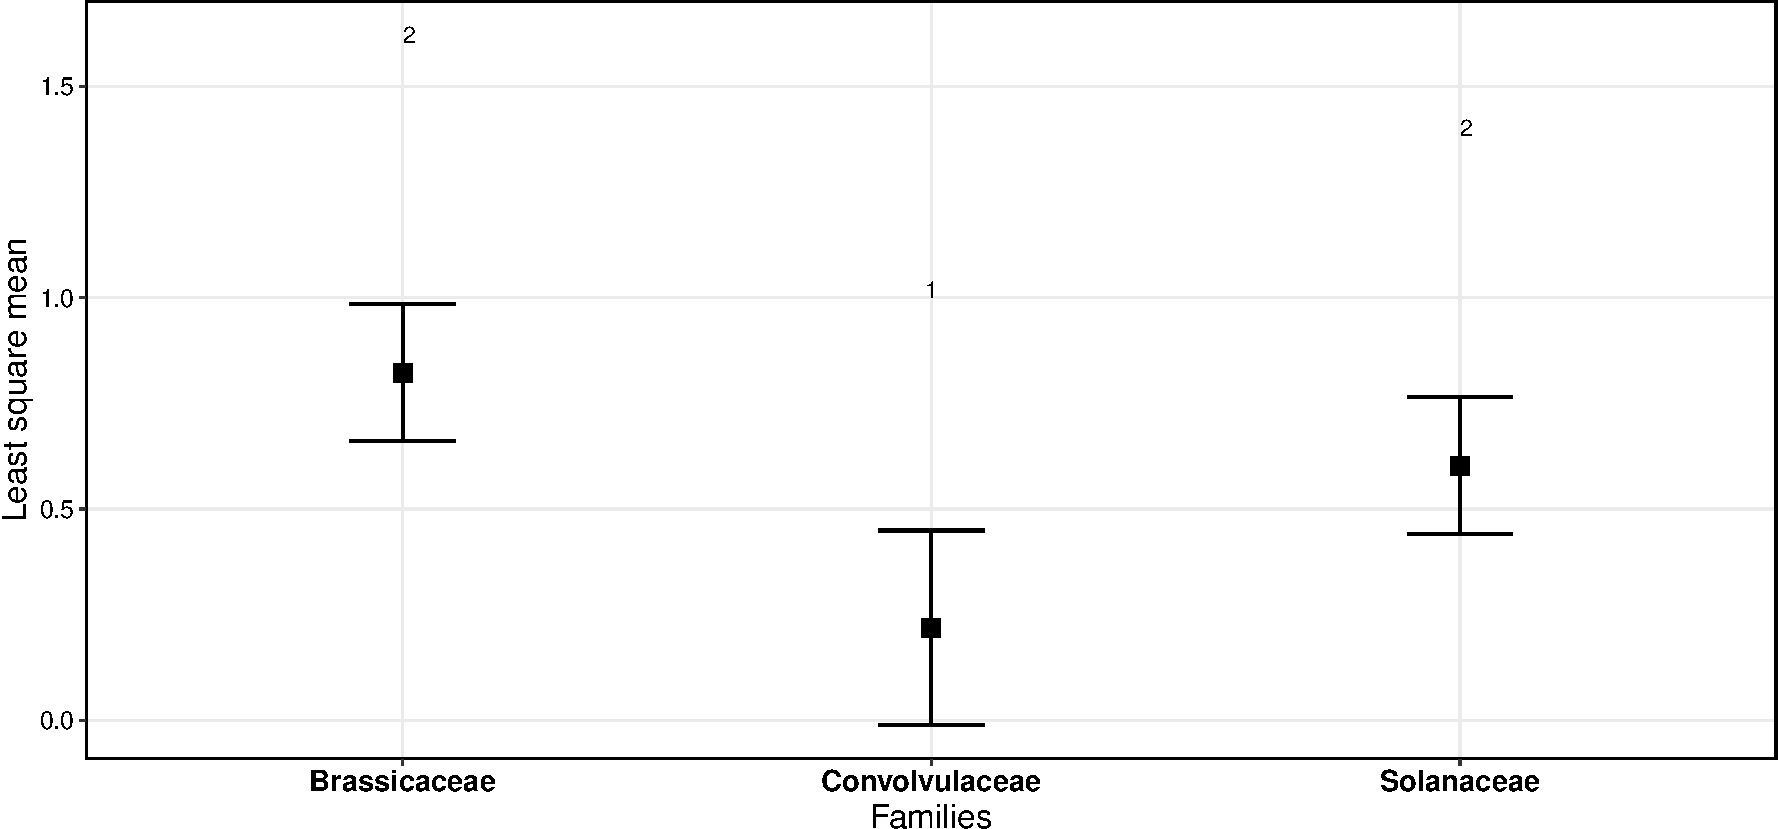
\includegraphics{Supp_Material_files/figure-latex/unnamed-chunk-7-1.pdf}
\caption{\textbf{Fig. S4} Pollen ratios comparisons between the
different pollen recipient families where the boxes represent least
square means, the error bars, confidence intervals 95\%, and sharing
numbers indicate no significant differences between groups (Tukey
adjusted comparisons). These pollen ratios (\%) are the total number of
heterospecific pollen grains divided by the total quantity of pollen
(conspecific pollen + heterospecific pollen), and then compared by
family (N=20). Brassicacea family is coloured in blue, Convolvulaceae in
green and Solanaceae in orange.}
\end{figure}

\newpage

\begin{figure}
\centering
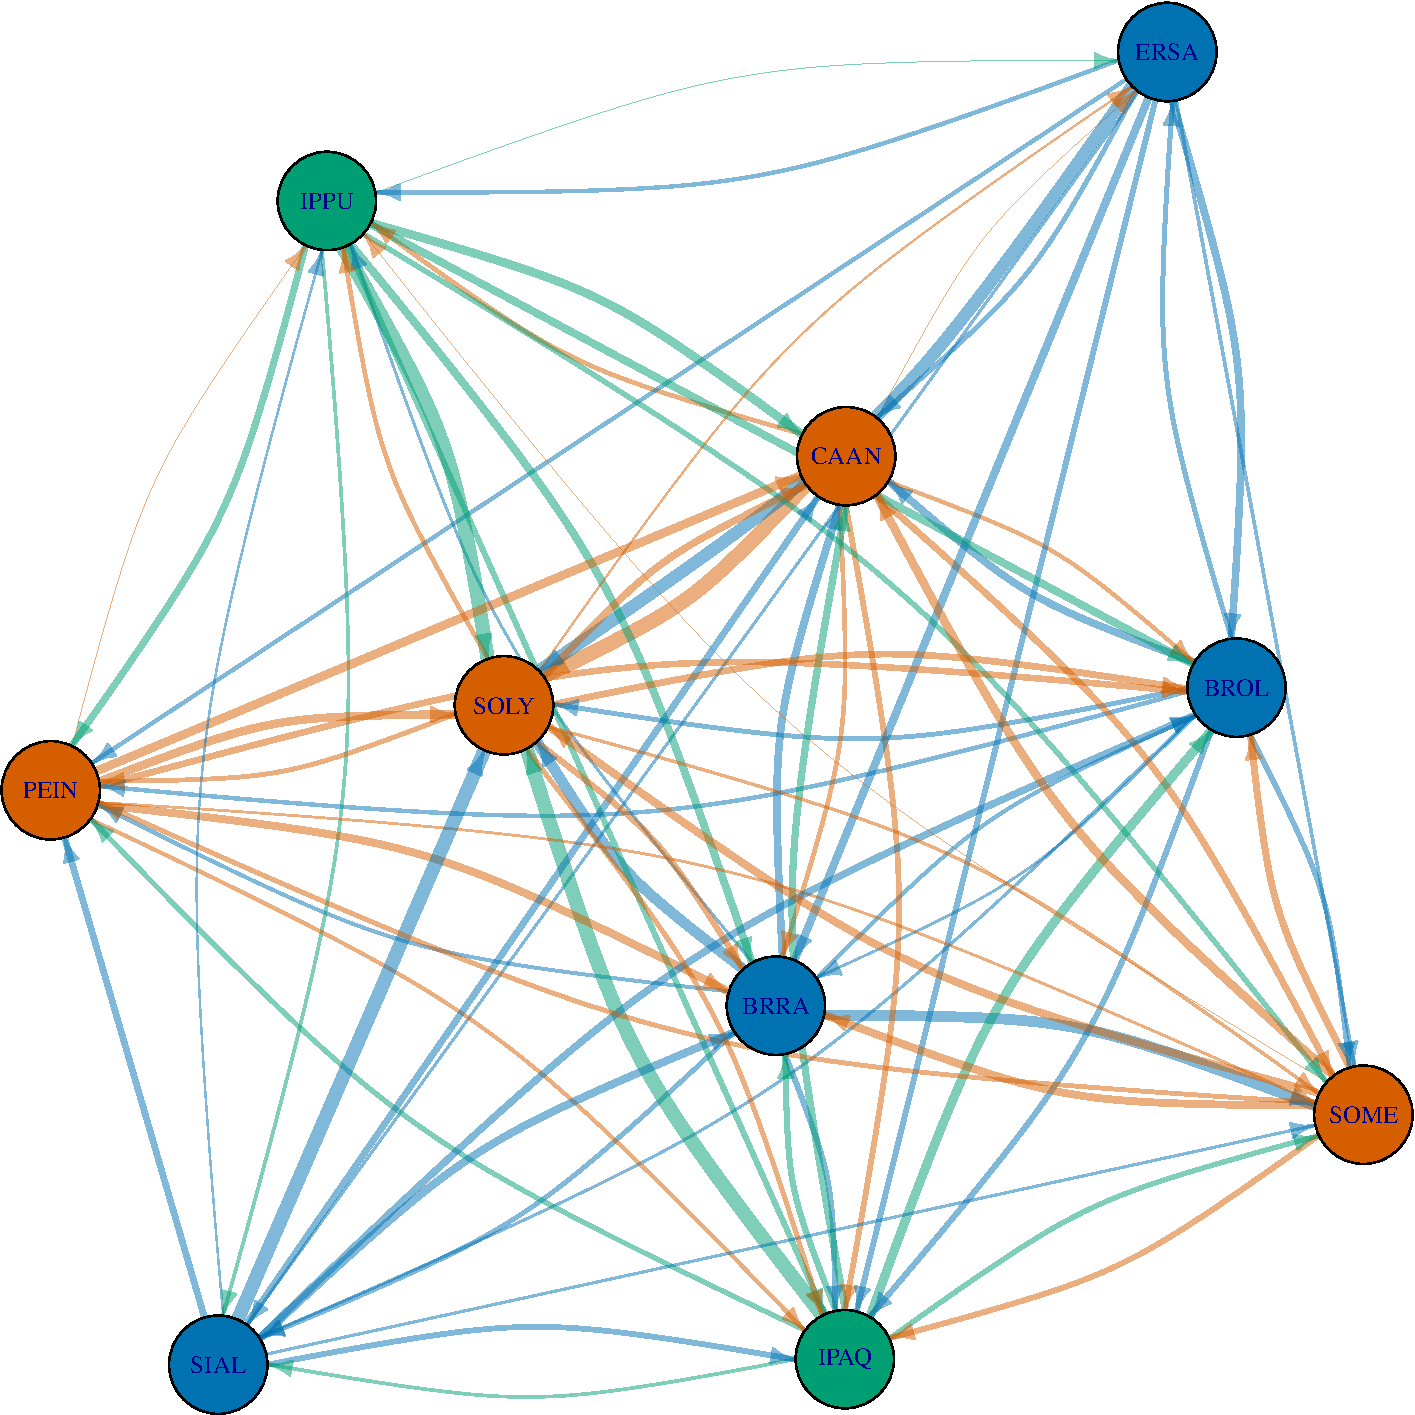
\includegraphics{Supp_Material_files/figure-latex/unnamed-chunk-8-1.pdf}
\caption{\textbf{Fig. S5} Unipartite bidirectional network with
asymmetrical effect. The lines with the arrow heads connect the impact
of foreign pollen (effect size) of each pollen donor species on each
recipient species. All the arrow heads point to the recipient species of
the reciprocal interaction. Lines of species that did not have a
negative impact are not represented. The different nodes and the effect
of the donor species on the recipient species appear coloured by family:
Solanaceae (orange), Brassicaceae (blue) and Convolvulaceae (green). The
intensity of the effect is represented by the line´s size where a larger
effect size corresponds to a thicker line and a thinner line to a
smaller effect size. Species code: BROL: Brassica oleracea, BRRA:
Brassica rapa, ERSA: Eruca sativa, SIAL: Sinapis alba, IPAQ: Ipomoea
aquatica, IPPU: Ipomoea purpurea, CAAN: Capsicum annuum, PEIN: Petunia
integrifolia, SOLY: Solanum lycopersicum, SOME: Solanum melongena.}
\end{figure}

\clearpage

\begin{figure}
\centering
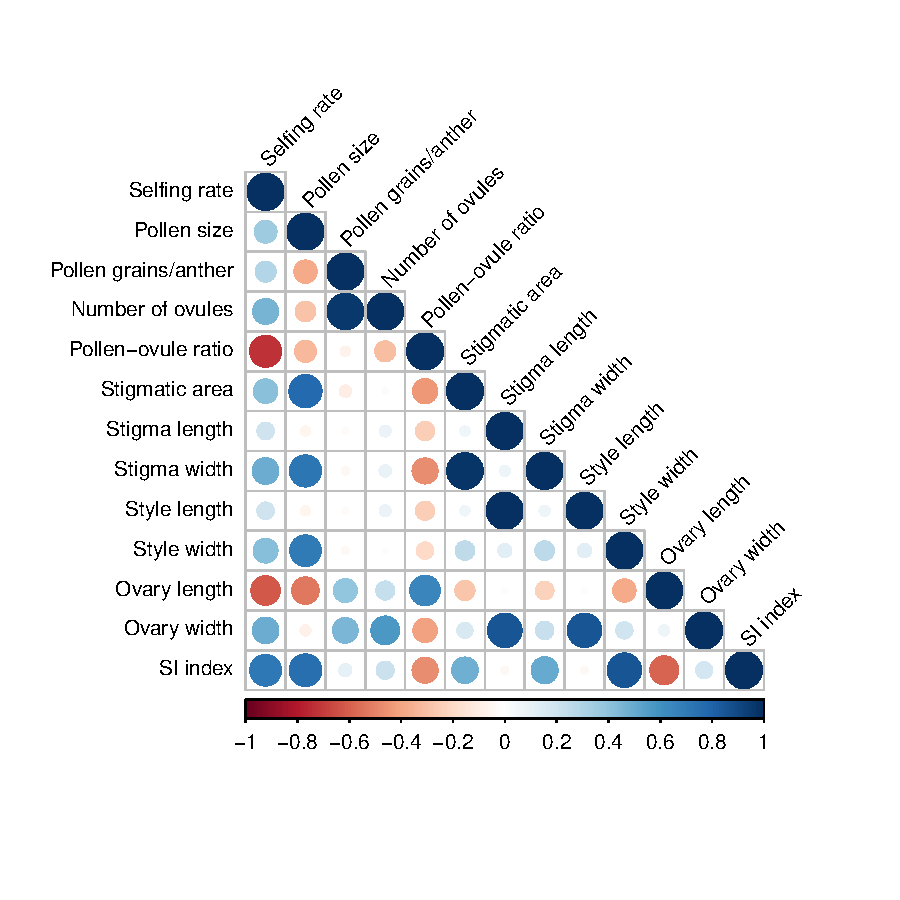
\includegraphics{Supp_Material_files/figure-latex/unnamed-chunk-9-1.pdf}
\caption{\textbf{Fig. S6} Graphical representation of the correlation
matrix of the different reproductive traits considered in the
experiment. Positive correlations are displayed in blue and negative in
red. The intensity, size and colour of the circles are proportional to
the correlation coefficient from Pearson's r.}
\end{figure}

\clearpage

\begin{figure}
\centering
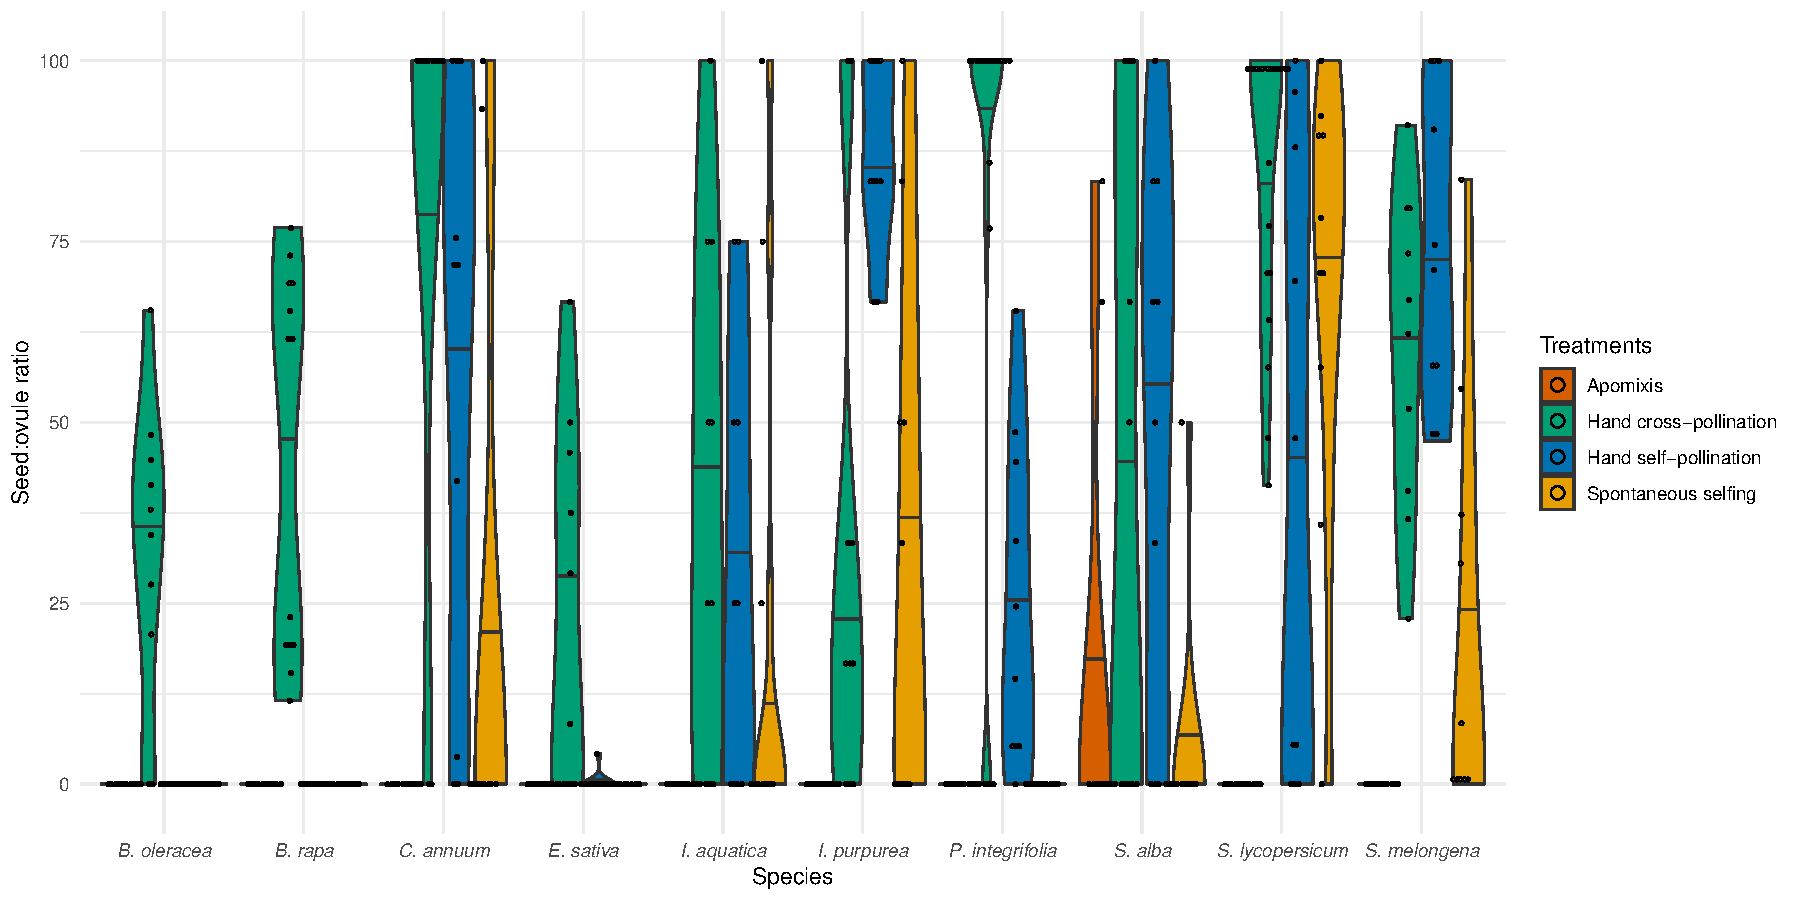
\includegraphics{Supp_Material_files/figure-latex/unnamed-chunk-10-1.pdf}
\caption{\textbf{Fig. S7} Violin plot of the proportion of seeds
coverted to ovule (\%) for all species with four different
hand-pollination treatments: apomixis (orange), hand cross pollination
(green), hand self pollination (blue) and spontaneous selfing (yellow).
The coloured dots, represent the different values of seed set for each
treatment.}
\end{figure}

\newpage

\begin{figure}
\centering
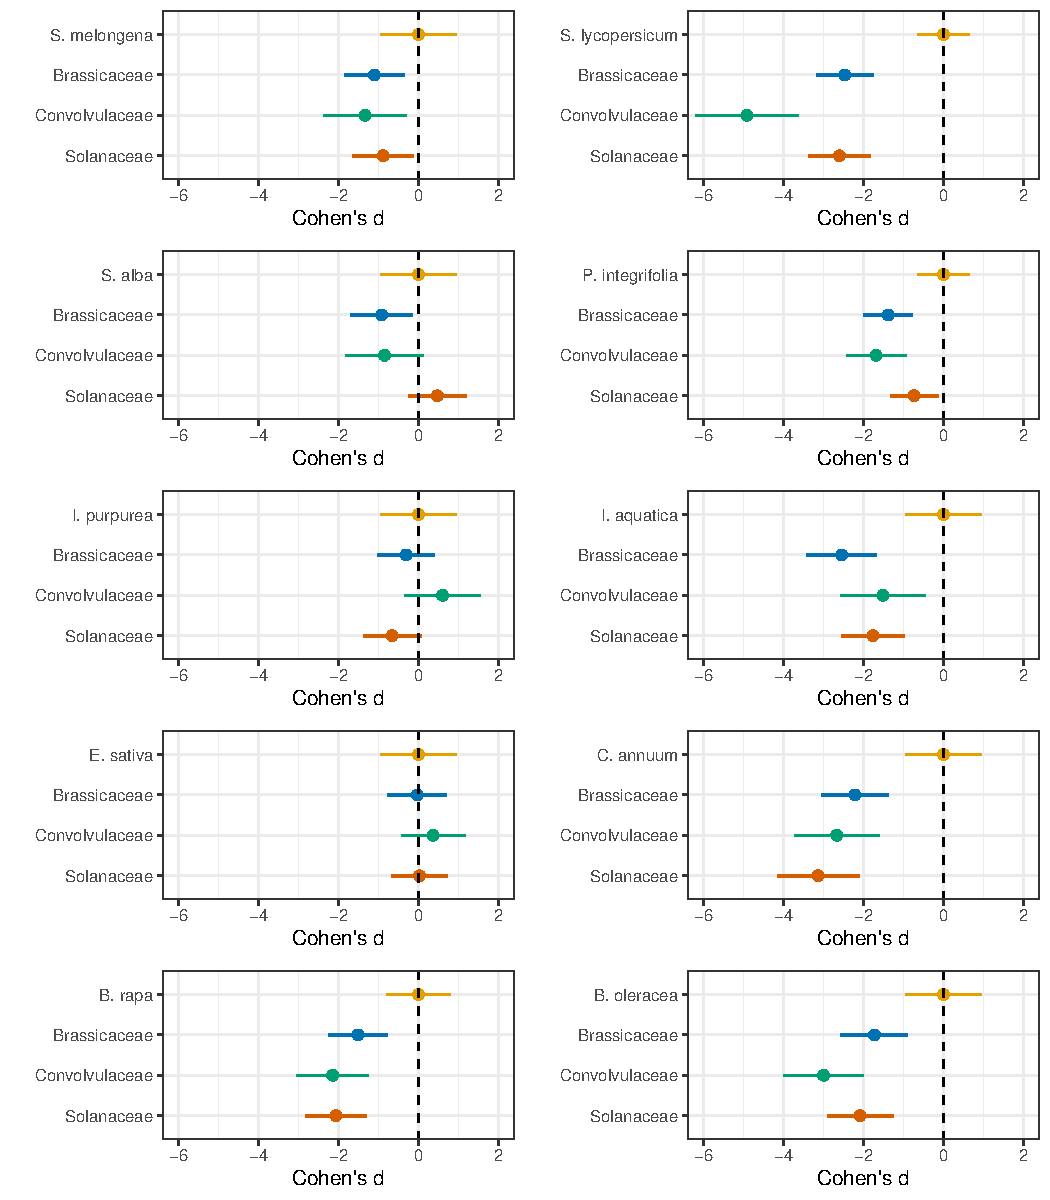
\includegraphics{Supp_Material_files/figure-latex/unnamed-chunk-11-1.pdf}
\caption{\textbf{Fig. S8} Grouped effect sizes (95\% confidence
intervals) of the different families on each focal species. For each
species, the grouped effect by family is compared with the control
treatment of hand cross pollination with conspecific pollen. The control
treatment is represented in yellow and vertically intersected with a
dashed line through the mean effect size in order to help the visual
interpretation of the effect sizes. Any value to the left of the
vertical dashed line represents a negative impact of foreign pollen. The
different effect sizes and confidence intervals are coloured by family:
Solanaceae (orange), Brassicaceae (blue) and Convolvulaceae (green).}
\end{figure}

\end{document}
